\documentclass[output=paper,
modfonts,
%bulgarian,greek,polish,portuguese,romanian,russian,english,hebrew
]{langscibook} 
%\bibliography{localbibliography}


\title{Preface} %Invent a better title 

\author{%
 Stella Markantonatou\affiliation{Institute for Language and Speech Processing, Athena RIC, Greece}\and 
 Carlos Ramisch\affiliation{Aix Marseille Univ, Université de Toulon, CNRS, LIS, Marseille, France}\and
 Agata Savary\affiliation{University of Tours, LIFAT, France}\lastand
 Veronika Vincze\affiliation{University of Szeged, Hungary}
}
\abstract{In this introductory chapter we present the rationale for the volume at hand. We explain the origin and the selection process of the contributing chapters, and we sketch the contents and the organization of the volume. We also describe notational conventions put forward for citing and glossing multilingual examples of multiword expressions. We finally acknowledge the efforts which paved the way for setting up this book project, ensuring its quality and publication.}%its quality assurance and its publication.}

\begin{document}

\maketitle
\rohead{Preface}

%The index of abbreviations in p.~\pageref{sec:abbreviations} gives the meaning of all language codes and of the grammatical codes used in glosses. 

%The preface is being drafted. For the time being we only include its most technical part so as to give guidelines to the authors about typesetting their linguistic examples.
%\sm{Stella's comment}
%\cara{Carlos' comment}
%\vv{Veronika's comment}
Multiword expressions (MWEs) belong to those language phenomena which pose the hardest challenges both in linguistic modelling and in automatic processing. This is due notably to their 
\is{non-compositionality!semantic}semantic non-compositionality, that is, %i.e. 
the impossibility to predict their meaning from their syntactic structure and from the semantics of their component words in a way deemed regular for the given language. But MWEs also exhibit unpredictable behaviour on other levels of language modelling such as the lexicon, morphology and syntax, and call, therefore, for dedicated procedures in natural language processing (NLP) applications.

These challenges have been addressed by an ever-growing and increasingly multilingual community  gathering at the Multiword Expressions Workshop, organized yearly since 2003, often jointly with major NLP conferences. 
The 13th edition of the Workshop, co-located with the EACL 2017 conference in Valencia, Spain, saw a major evolution of the topics and methods addressed by the community. This evolution resulted notably from the efforts coordinated by \isi{PARSEME}, a European research network dedicated to parsing and MWEs, gathering, since 2013,  researchers from 31 countries and working on as many languages.\footnote{\url{http://www.parseme.eu}} %\vv{Shall we put the footnote to the end of the sentence?}

One of \isi{PARSEME}'s main outcomes was a corpus in 18 languages annotated for verbal MWEs (VMWEs), based on a unified methodology and terminology, % according to unified terminologies and methodologies, 
and published under open licenses. This considerable collective and inclusive effort mobilized experts from different linguistic traditions, triggered cross-language and cross-domain discussions, and brought convergence to modelling and processing of MWE-related phenomena. The availability of this %the 
new open resource also made it possible to organize the 
\is{PARSEME!shared task}PARSEME Shared Task on Automatic Identification of Verbal Multiword Expressions, i.e. a competition of VMWE identification tools, whose culminating event was hosted by the MWE 2017 workshop in Valencia. The 7 participating systems covered jointly all 18 languages represented in the corpus. They also offered a large panorama of 
\is{multiword expression!identification}VMWE identification techniques. These assets, as well as some other contributions published in the main track of the MWE 2017 workshop, showed a growing awareness by the MWE community of specific challenges posed, in particular, 
%notably \sm{the adverb \textit{notably} has been  used 3 times so far} 
by verbal MWEs, such as their discontinuity and high morpho-syntactic flexibility. The workshop programme addressed a large variety of MWE-dedicated tasks such as: lexical and grammatical encoding, annotation, tokenization, extraction, identification, classification, variation study, parsing, compositionality prediction, and translation. Finally, it testified that MWE research has reached a highly multilingual stage. 

%%%%%%%%%%%%%%%%%%%%%%%%%%%
\section{Organization and contents of the volume}
\largerpage
This volume is a collection of selected extended papers from the MWE 2017 workshop in Valencia: 8 of them from the main track, and 5 from the \is{PARSEME!shared task}shared task track. They address 19 languages from 9 language families, as shown in \figref{preface:fig:language-tree}. 
%\footnote{When specific dialects of these languages are addressed (e.g.~Brazilian Portuguese), they are explicitly mentioned in the language index (cf.~\pageref{??}).}
%\sm{Which language index is this? Is it section 4 in this introductory chapter that gives abbreviations or is it the language index of the book  which says the pages where each language is mentioned?}
The chapter selection process was initiated by an open call, addressed to all co-authors of the workshop papers. The call included %and including
the requirement of extending the original contributions by at least 30\% with unpublished content. An %The 
international programme committee reviewed 15 submissions and selected 14 of them for publication. One of the selected chapters was further withdrawn. As a result, the volume consists of 13 chapters covering a large variety of aspects related to  MWE representation and processing, with a particular focus on verbal MWEs.


\begin{figure}
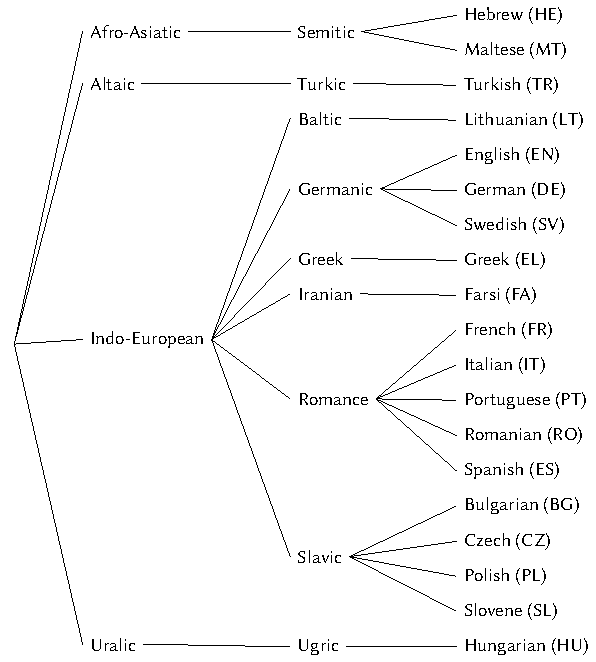
\includegraphics[width=0.70\textwidth]{figures/language-tree.pdf}
\caption{Languages addressed in the chapters of this volume, together with their two-letter language code, language families and genera (middle columns), according to WALS (World Atlas of Language Structures, ~\citealt{wals13}).}
%, \url{http://wals.info/}.}
\label{preface:fig:language-tree}
\end{figure}
%\todo[inline]{CR: something missing here. ``genera'' what?}


%Baltic (\ili{Lithuanian}), Germanic (\ili{English}, \ili{German} and \ili{Swedish}), \ili{Greek} (\ili{Greek}), Iranian (\ili{Farsi}), Romance (\ili{French}, \ili{Italian}, \ili{Portuguese}, \ili{Romanian} and \ili{Spanish}), Semitic (\ili{Hebrew} and \ili{Maltese}), Slavic (\ili{Bulgarian}, \ili{Czech}, \ili{Polish} and \ili{Slovene}), Turkic (\ili{Turkish}), and Ugric (\ili{Hungarian}).




%\as{Mention the workshop. \isi{
%Mention \isi{PARSEME}.
%Address the specific challenges behind verbal MWEs. Breakthrough in this domain via the \isi{PARSEME} \isi{corpus} \isi{annotation} project and the \isi{shared task}. Stress the huge collective and highly multilingual effort. MWE research is now more deeply grounded in the multilingual data. }

%The first three chapters 
Chapters 1 %\ref{GEERAERT-CHAPTER} 
to 3 %\ref{BHATIA-CHAPTER}
address outstanding linguistic properties of VMWEs and their automatic assessment. \citetv{Geeraerttv}  discuss \is{idiomatic variation}idiomatic \emph{variation} of several types of \ili{English} verbal idioms. They %assess its \isi{acceptability} via psycholinguistic experiments based on rating and eye-tracking experiments 
draw on multimodal evidence, namely \is{idiomatic variation!acceptability}acceptability rating and \isi{eye-tracking} measurements, to investigate \is{idiomatic variation!comprehension}comprehension mechanisms. \citetv{Barancikovatv} deal with light-verb constructions and verbal idioms in \ili{Czech}, and explore their \is{verbal multiword expression!paraphrasability}paraphrasability by single verbs. They also propose a lexicographic scheme for VMWE paraphrase encoding, and show its usefulness in \isi{machine translation}. \citetv{Bhatiatv}  focus on \ili{English} verb-particle constructions, and estimate their compositionality\is{compositionality} degree, so as to further compute the semantics of sentences containing verb-particle constructions %VPCs, 
on the basis of lexical, grammatical and ontological resources.

\newpage 
Chapters 4 %\ref{SAVARY-CHAPTER} 
to 8 %\ref{SIMKO-CHAPTER} %\sm{needs to be taken care of when the whole book is compiled} 
are dedicated to the \is{PARSEME!shared task}PARSEME shared task on automatic identification of verbal MWEs. \citetv{Savarytv} describe %address 
the \is{PARSEME!corpus}PARSEME multilingual VMWE-annotated corpus underlying the shared task. In a first step, the annotation guidelines\is{annotation!guidelines} and methodology are presented, then 
%\sm{I would use \textit{as well as} if an \textit{and} connecting verbs  existed. However, the existing \textit{and} connects nouns.} 
the properties of the annotated corpus are analysed across the 18 participating languages. \citetv{Maldonadotv} offer a critical analysis of the shared task organization and of its results across languages and participating systems. Chapters 6 to 8 %Chapters MOREAU-CHAPTER--ALSAIED-CHAPTER 
are dedicated to three of the seven %7
\is{multiword expression!identification}VMWE identification systems participating in the shared task. They show a representative panorama of recent techniques used to address the VMWE identification task. \citetv{Moreautv}  model the task as \isi{sequence labelling} with \isi{reranking}. \citetv{Simkotv}  rely on a generic \is{parsing!dependency}dependency parser trained on a corpus with merged syntactic and VMWE labels. Finally, \citetv{AlSaiedtv} present a dedicated \is{parsing!transition-based}transition-based dependency parser, which jointly predicts a syntactic dependency tree and a forest of VMWEs. 

Chapters 9 %\ref{BROOKE-CHAPTER} 
to 11 %\ref{TASLIMIPOOR-CHAPTER} 
further discuss \is{multiword expression!identification}MWE identification issues in various settings and scopes. \citetv{Brooketv} show how comparing various annotations of the same MWE in an \ili{English} corpus can help correct annotation errors, enhance the \is{annotation!consistency}consistency of corpus annotation, and consequently increase the quality of downstream MWE identification systems. \citetv{Scholivettv} address identification of \ili{French} continuous MWEs via \isi{sequence labelling}, compare its results to more sophisticated parsing-based approaches, and show that feature engineering based on external lexical data (whether hand-crafted or automatically extracted) systematically enhances the tagging performance. \citetv{Taslimipoortv}, conversely, advocate 
%in favor \sm{either \textit{argue in favor} or \textit{advocate}} of 
modelling MWE identification as \isi{classification} rather than tagging\is{sequence labelling}. They exploit \isi{word embeddings} as classification features in \ili{Italian}, \ili{Spanish} and \ili{English}, and put forward a MWE-specific methodology of train vs.~test corpus split.

The last two chapters of the book, 12 %\ref{GARCIA-CHAPTER} 
and 13, %\ref{SALEHI-CHAPTER}, %this volume % TO AVOID PAGE OVERFLOW of "MWE-oriented"
are dedicated to multilingual MWE-oriented applications. \citetv{Garciatv} describes automatic extraction of bilingual \isi{collocation} equivalents in \ili{English}, \ili{Spanish}, and \ili{Portuguese}, using syntactic dependencies, association measures and distributional models. Finally, \citetv{Salehitv}  predict the \isi{compositionality} of \ili{English} and \ili{German} MWEs on the basis of their translations extracted from highly multilingual lexical resources. 

%\as{Explain how the volume is organized (add a sentence about each chapter), i.e. chapter clusters: (i) more linguistic papers which discuss the nature of MWEs and provide background for more computationally-oriented papers; within papers of the same type, we use alphabetical order, (ii) verbal MWEs: 12, 5, 10, 9, (iii) \isi{shared task} papers: 
%general descriptions: 15 (\isi{corpus}), 3 (Maldonado); system papers (in alphabetical order of the first authors): 4 (Moreau), 14 (Hazem), 7 (Simko), (iv) MWE \isi{identification}: 2, 8, (v) MWE translations: 1, 6? (multilingual resources).}

%%%%%%%%%%%%%%%%%%%%%%%%%%%
%\section{Open resources released in connection to the volume}

%Additionally to the important research questions mentioned above, this volume also address the major bottleneck in NLP research and technology, namely insufficiency of language resources. Several chapters offer various types of MWE resources in various languages, available under open licenses. 
%BARANCIKOVA-CHAPTER-CITE introduce ParaDi, a \isi{syntactic} dictionary of VMWE paraphrases in \ili{Czech}.

%Finally, SAVARY-CHAPTER-CITE address the \isi{PARSEME} VMWE-annotated \isi{corpus} in 18 languages, as discussed above. This resource has its follow-up including 20 languages, published for the needs of edition 1.1 of the \isi{PARSEME} \isi{shared task},\footnote{\url{http://multiword.sourceforge.net/sharedtask2018}} during the editorial work on this volume.

%Research described by some chapters of this volume resulted in linguistic resources available under open licenses. BARANCIKOVA-CHAPTER-CITE in



%%%%%%%%%%%%%%%%%%%%%%%%%%%
\section{Conventions for citing and glossing multilingual MWE examples}
%\section{Notational conventions}

 As mentioned above, this volume addresses a large number of languages, particularly in the chapters related to the PARSEME corpus and shared task. Therefore, the editorial effort around this volume includes putting forward \is{multiword expression!notational conventions}notational conventions which might become a standard for citing and glossing multilingual MWE examples.
%Some chapters cite MWE examples in several languages. These multilingual \emph{numbered examples}, as (\ref{preface:en:take-on}) to (\ref{preface:fa:have-sleep-for-sb}), contain: 
We illustrate the proposed conventions by the \emph{numbered examples}  (\ref{preface:en:take-on}) to (\ref{preface:fa:have-sleep-for-sb}). Each numbered example contains:%They  contain:
\begin{enumerate}[(i)]%[label=(\roman*)]
\item\label{ex-line:use} a sample use of the VMWE, followed by the 2-letter ISO 639-1 language code (cf.~\figref{preface:fig:language-tree}),
%(cf. the list of abbreviations p.~\pageref{sec:lang-codes}),\sm{if we retain section four for the codes, should the reference be that of a section?}

\item\label{ex-line:transcription} a transcription, if the language of the example is written with a script different from the one used for the main text,\footnote{For instance, transcription is needed for Bulgarian, Greek, Farsi and Hebrew examples in this volume. Conversely, examples in English, or any other language using Latin script, would require transcriptions %be needed 
in texts written in Cyrillic, Greek, Arabic or Hebrew script.}
%a non-Latin alphabet, 
%\sm{Well, this is a very "Stella-like" comment: I would suggest something like \textit{if a language has is written with an alphabet different than the alphabet used for the main text (the main text of this book is written in the Latin alphabet)} because the scripture of a language is part of a nation's identity rather than being a kind of deviation from the norm, something that might be inferred from the existing wording; as I said, this is a very Stella-like comment and you might find it exaggerated.}


\item\label{ex-line:gloss} a gloss %according to 
following 
the Leipzig Glossing Rules,\footnote{\url{https://www.eva.mpg.de/lingua/pdf/Glossing-Rules.pdf}} 

\item\label{ex-line:trans} a \isi{literal translation}, followed by an \isi{idiomatic translation} in single quotes. 
\end{enumerate}

For \ili{English} examples, items (\ref{ex-line:transcription})--(\ref{ex-line:trans}) are irrelevant or optional but \isi{idiomatic translation} might sometimes be useful to ease the comprehension by non-native readers. For right-to-left languages (e.g. \ili{Farsi} or \ili{Hebrew}), item (\ref{ex-line:use}) is spelled right-to-left, item (\ref{ex-line:trans}) left-to-right and items (\ref{ex-line:transcription})--(\ref{ex-line:gloss}) left-to-right within components, and right-to-left from one component to another. 
Lexicalized components of the VMWE, i.e. those which are always realized by the same lexeme %(cf. \citealtv{Savarytv}:~\pageref{sec:def-scope}) 
(cf. \citealtv{Savarytv}, \sectref{sec:def-scope}, p. \pageref{sec:def-scope}) 
are highlighted in bold face. 

%\begin{exe}


\ea\label{preface:en:take-on}
\settowidth \jamwidth{(EN)} 
She reluctantly \lex{took} \lex{on} this task. \jambox{(EN)}
\glt `She reluctantly agreed to be in charge of this task.'
\z

\ea \label{preface:sl:skrivati-glavo-v-pesek}
\settowidth \jamwidth{(SL)} 
\gll Ida \lex{skriva} \lex{glavo} \lex{v} \lex{pesek}. \\
Ida hide.\textsc{3.sg} head in sand \\ \jambox{(SL)}
% Eva thrusts head in sand \\
\glt Ida hides her head in the sand. `Ida pretends not to see a problem.’
\z

\ea \label{preface:el:take-decision}
\settowidth \jamwidth{(EL)} 
\glll Η Ζωή \lex{παίρνει} μία \lex{απόφαση}. \\
i Zoi perni mia apofasi \\
the\textsc{.fem.sg} Zoe\textsc{.fem.sg} take.\textsc{3.sg} a decision \\ 
\jambox{(EL)}
\glt Zoe takes a decision. `Zoe makes a decision.'
\z

\ea \label{preface:fa:have-sleep-for-sb}
\settowidth \jamwidth{(FA)} 
\glll \PRL{است} \lex{\PRL{دیده}} \lex{\PRL{خواب}} \PRL{من} \lex{\PRL{برای}} \PRL{کافی} \PRL{قدر} \PRL{به} \\
%æst di:de xɒ:b mæn bærɒ:je kɒ:fi: qædre be  \\
ast \lex{dide} \lex{khab} man \lex{baraye} kafi qadre be  \\
is seen sleep me for enough quantity to\\ \jambox{(FA)}
\glt He had enough sleep for me. `He has many plans for me.’
\z

%\end{exe}

%These examples are to be typeset by the dedicated LSP commands, e.g. example (\ref{preface:el:take-decision}) is typeset like this:

%\begin{verbatim}
%\ea \label{preface:el:take-decision}
%\settowidth \jamwidth{(EL)} 
%\glll Η Ζωή \lex{παίρνει} μία \lex{απόφαση}. \\
%i zoi perni mia apofasi \\
%the\textsc{.fem.sg} Zoe\textsc{.fem.sg} take.\textsc{3.sg} a decision \\ 
%\jambox{(EL)}
%\glt Zoe takes a decision. `Zoe makes a decision.'
%\z
%\end{verbatim}


\emph{In-line examples}, used for brevity, are preceded by the 2-letter language code, contain items (\ref{ex-line:use}), (\ref{ex-line:transcription}) if relevant, and (\ref{ex-line:trans}) only, and the \isi{idiomatic translation} (if any) is introduced by a double arrow `$\Rightarrow$'. For instance, an in-line example corresponding to numbered example (\ref{preface:sl:skrivati-glavo-v-pesek}) would be the following: (SL) \exlitidio{Ida \lex{skriva} \lex{glavo} \lex{v} \lex{pesek}}{Ida hides her head in the sand}{Ida pretends not to see a problem}. 
%
If the language under study is written with a non-Latin alphabet, the inline example should not be in italics, and the transliteration should be included in parentheses, e.g. (EL) \nlextlilitidio{Η Ζωή \lex{παίρνει} μία \lex{απόφαση}}{I Zoi perni mia apofasi}{The Zoe takes a decision}{Zoe makes a decision}. To keep such examples reasonably short, the first item can be omitted and only the transliterated example is kept: (EL) \nltlilitidio{I Zoi perni mia apofasi}{The Zoe takes a decision}{Zoe makes a decision}. 
%
The literal or the \isi{idiomatic translation} are sometimes superfluous or too verbose, and can be skipped, as in:  (EL) \nltliidio{I Zoi perni mia apofasi}{Zoe makes a decision}. 

The typesetting commands for both numbered and in-line examples for {\LaTeX} can be found in the GitHub repository containing the source codes of this volume, accessible from its webpage.\footnote{\url{http://langsci-press.org/catalog/book/204}} %TO CHECK!!!!!!!!!!!!!!!!!!!!!!!!!!!!!!!

%In-line examples are to be typeset by commands specific to this volume, defined in the \texttt{localcommands.tex} file. For instance, the four last examples are typeset as follows:

%\begin{small}
%\begin{verbatim}
%(SL) \exlitidio{Ida \lex{skriva} \lex{glavo} \lex{v} \lex{pesek}}
%{Ida hides her head in the sand}{Ida pretends not to see a problem} 
%(EL) \nlextlilitidio{Η Ζωή \lex{παίρνει} μία \lex{απόφαση}}
%{I zoi perni mia apofasi}{The Zoe takes a decision}{Zoe makes a decision}
%(EL) \ntlilitidio{I zoi perni mia apofasi}{Zoe takes a decision}
%{Zoe makes a decision}
%(EL) \nltliidio{I zoi perni mia apofasi}{Zoe makes a decision
%\end{verbatim}
%\end{small}

%In each usage example the head verb is either in a finite form or in the infinitive (only when the subject is not lexicalized). 



%We put forward these conventions as a future notation standard for multilingual examples of MWEs.
%\as{Dialects are indexed separately.}

%%%%%%%%%%%%%%%%%%%%%%%%%%%
\section{Acknowledgements}
Huge collective efforts paved the way towards the publication of this volume. 

The \is{PARSEME!shared task} PARSEME Shared Task on Automatic Identification of VMWEs was made possible by the European research network \isi{PARSEME}\footnote{\url{http://www.parseme.eu}}, funded by the IC1207 COST\footnote{\url{http://www.cost.eu/}} Action in 2013--2017. The PARSEME core group and eighteen language teams (cf.~acknowledgements in \citealtv{Savarytv}) prepared the annotation guidelines and tools, and created the multilingual \is{PARSEME!corpus}corpus underlying the shared task. We are also grateful to the COST Officials, notably to Ralph Stübner, for their %his
continuous support in the scientific and financial administration of the Action. 

The \is{MWE 2017 workshop}13th Workshop on Multiword Expressions (MWE 2017)\footnote{\url{http://multiword.sourceforge.net/mwe2017}}  was organized and sponsored by PARSEME jointly with the Special Interest Group on the Lexicon (\isi{SIGLEX})\footnote{\url{http://siglex.org/}} of the Association for Computational Linguistics. An international Programme Committee of over 80 researchers from 27 countries reviewed the workshop submissions and ensured a high-quality paper selection.

Our warm acknowledgements go also to the Editorial Staff of Language Science Press, and in particular to Sebastian Nordhoff, for his expert and friendly  editorial assistance. We are also grateful to the editors of the \emph{Phraseology and Multiword Expressions} book series for their support. In particular, Yannick Parmentier played the role of the editor-in-charge of the volume, and offered advice on technical editorial issues.

Finally, we thank the following reviewers, who provided insightful reviews to the chapters submitted to this volume:

\begin{itemize}
\item Dimitra Anastasiou (Luxembourg Institute of Science and Technology,\\ Luxembourg)
\item Doug Arnold (University of Essex, UK)
\item Timothy Baldwin (University of Melbourne, Australia)
\item Eduard Bejček (Charles University in Prague, Czech Republic)
\item António Branco (University of Lisbon, Portugal)
\item Marie Candito (Paris Diderot University, France)
\item Fabienne Cap (Uppsala University, Sweden)
\item Matthieu Constant (Université de Lorraine, France)
\item Paul Cook (University of New Brunswick, Canada)
\item Lucia Donatelli (Georgetown University, USA)
\item Silvio Ricardo Cordeiro (Aix-Marseille University, France)
\item Béatrice Daille (University of Nantes, France)
\item Gaël Dias (University of Caen Basse-Normandie, France)
\item Voula Giouli (Institute for Language and Speech Processing/Athena RIC, Greece)
\item Tracy Holloway King (eBay, USA)
\item Philipp Koehn (Johns Hopkins University, USA)
\item Dimitrios Kokkinakis (University of Gothenburg, Sweden)
\item Yannis Korkontzelos (Edge Hill University, UK)
\item Eric Laporte (Université Paris-Est Marne-la-Vallee, France)
\item Timm Lichte (University of Düsseldorf, Germany)
\item Gyri S. Losnegaard (University of Bergen, Norway)
\item Héctor Martínez Alonso (Thomson Reuters Labs, Canada)
\item Verginica Mititelu (Romanian Academy Research Institute for Artificial Intelligence, Romania)
\item Preslav Nakov (Qatar Computing Research Institute, HBKU, Qatar)
\item Joakim Nivre (Uppsala University, Sweden)
\item Jan Odijk (University of Utrecht, Netherlands)
\item Petya Osenova (Bulgarian Academy of Sciences, Bulgaria)
\item Harris Papageorgiou (Institute for Language and Speech Processing/Athena RIC, Greece)
\item Yannick Parmentier (Université de Lorraine, France)
\item Carla Parra Escartín (Dublin City University, ADAPT Centre, Ireland)
\item Agnieszka Patejuk (Institute of Computer Science, Polish Academy of Sciences, Poland)
\item Pavel Pecina (Charles University in Prague, Czech Republic)
\item Scott Piao (Lancaster University, UK)
\item Martin Riedl (University of Stuttgart, Germany)
\item Manfred Sailer (Goethe-Universität Frankfurt am Main, Germany)
\item Nathan Schneider (Georgetown University, USA)
\item Sabine Schulte Im Walde (University of Stuttgart, Germany)
\item Ruben Urizar (University of the Basque Country, Spain)
\item Aline Villavicencio (Federal University of Rio Grande do Sul, Brazil)
\item Jakub Waszczuk (University of Tours, France)
\item Shuly Wintner (University of Haifa, Israel)
\end{itemize}

We hope that the quality of this volume will be a valuable reward to all these contributors, and a source of information and inspiration for the international MWE community.

\begin{comment}
%%%%%%%%%%%%%%%%%%%%%%%%%%%
\section{Language codes}
\label{sec:lang-codes}

%Whenever chapters of this volume cite linguistic examples in several languages, those examples are annotated with the following 2-letter ISO 639-1 language codes.
Annotations with the following 2-letter ISO 639-1 codes indicate the language of the examples used in this book.

\begin{table}
\begin{tabularx}{.45\textwidth}{ll}
%\sout{AR} & Arab \\
\textsc{BG} & \ili{Bulgarian} \\
\textsc{CS} & \ili{Czech} \\
\textsc{DE} & \ili{German} \\
\textsc{EL} & \ili{Greek} \\
\textsc{EN} & \ili{English} \\
\textsc{ES} & \ili{Spanish} \\
\textsc{ET} & Estonian \\
%\sout{EU} & Basque \\
\textsc{FA} & \ili{Farsi} \\
\textsc{FR} & \ili{French} \\
\textsc{HE} & \ili{Hebrew} 
%\sout{HI} & Hindi \\
%\textsc{HR} & Croatian 
\end{tabularx}
\begin{tabularx}{.45\textwidth}{ll}
\textsc{HU} & \ili{Hungarian} \\
%\sout{ID} & Indonesian\\
%\sout{JA} & Japanese \\
\textsc{IT} & \ili{Italian} \\
\textsc{LT} & \ili{Lithuanian} \\
\textsc{MT} & \ili{Maltese} \\
\textsc{PL} & \ili{Polish} \\
\textsc{PT} & \ili{Portuguese} \\
\textsc{RO} & \ili{Romanian} \\
\textsc{SL} & \ili{Slovene} \\
\textsc{SV} & \ili{Swedish} \\
\textsc{TR} & \ili{Turkish} 
%\textsc{YI} & Yiddish \\
%\sout{ZH} & Chinese 
\end{tabularx}
\end{table}
\end{comment}

\sloppy
\printbibliography[heading=subbibliography,notkeyword=this]


\end{document}
